\documentclass[11pt]{book}

\usepackage{fullpage}
\usepackage{graphicx}
\usepackage{cite}
\usepackage{times}
\usepackage{url}
\usepackage{setspace}
\usepackage{fancyhdr}
\usepackage{ifthen}
\usepackage{listings}
\usepackage{color}
\usepackage[section]{placeins}
\usepackage{xtab}
\usepackage{url}
\usepackage[ruled]{algorithm2e}
%\usepackage{hyperref}

\setcounter{topnumber}{2}
\setcounter{bottomnumber}{3}
\setcounter{totalnumber}{4}
\renewcommand{\topfraction}{0.5}
\renewcommand{\bottomfraction}{0.95}
\renewcommand{\textfraction}{0.1}
\renewcommand{\floatpagefraction}{0.7}

\setlength{\abovecaptionskip}{3pt}
\setlength{\belowcaptionskip}{3pt}

\pagestyle{fancy}
\setboolean{@twoside}{false}
\setlength{\headsep}{25pt}
\setlength{\headheight}{14pt}

\newcommand{\showPlots}[3]{
  \begin{figure}
    \begin{minipage}{.5\textwidth}
      \begin{center}
        \includegraphics[width=\textwidth,keepaspectratio]{figs/traffic/#1} \\
        Traffic Model \\
      \end{center}
    \end{minipage} \hfill \begin{minipage}{.5\textwidth}
      \begin{center}
        \includegraphics[width=\textwidth,keepaspectratio]{figs/pcs/#1} \\
        PCS Model \\
      \end{center}
    \end{minipage}
    \caption{#3}\label{#2}
  \end{figure}
}

\definecolor{dkgreen}{rgb}{0,0.6,0}
\definecolor{gray}{rgb}{0.5,0.5,0.5}
\definecolor{mauve}{rgb}{0.58,0,0.82}

\lstset{frame=tb,
  language=C++,
  columns=flexible,
  basicstyle={\linespread{0.9}\small\ttfamily},
  breaklines=true,
  captionpos=b,
  aboveskip=0.2in,
  belowskip=0.2in,
  numberstyle=\tiny\color{gray},
  keywordstyle=\color{blue},
  commentstyle=\color{dkgreen},
  stringstyle=\color{mauve},
  tabsize=4
}

\begin{document}

\thispagestyle{empty}

\doublespacing

\vspace*{0.5in}

\begin{center}
\LARGE{\textbf{Time Warp Simulation on Multi-core Processors and Clusters}}

\vspace*{0.4in}

  {\large A thesis submitted to the\\[0.20in]
    Division of Research and Advanced Studies\\
    of the University of Cincinnati\\[0.20in]
    in partial fulfillment of the\\
    requirements for the degree of\\[0.20in]
    \textbf{MASTER OF SCIENCE}\\[0.20in]
    in the School of Electric and Computing Systems\\
    of the College of Engineering and Applied Sciences\\[0.20in]
    August xx, 2015\\[0.20in]
    by\\[0.20in]
    \textbf{Doug Weber}\\
    BSEE, University of Cincinnati, 2014\\}
  \vspace{0.5in}
  {\large Thesis Advisor and Committee Chair:  Dr. Philip A. Wilsey}
\end{center}

\clearpage

\setcounter{page}{1}
\pagenumbering{roman}
\clearpage

\chapter*{Abstract} 

%% the abstract covers your thesis soup to nuts.  the abstract may be published
%% separately from the main body so it needs to be fully contained and say
%% something about nearly everything in your thesis.  basically in 1-2 pages you
%% need to: bring the reader into your topic, explain why it is important and
%% why existing solutions are insufficient, it must describe your approach to a
%% solution and what your primary results are.  whew!!

\chapter*{Acknowledgments} 

%% put your acknowledgements here.

%% these three lines will cause latex to automatically generate these entries
%% for you....nice.  you can comment them out if, for example, your thesis does
%% not contain any tables.
\tableofcontents \markright{ }
\listoffigures \markright{ }
%\listoftables \markright{ }
\listofalgorithms \markright { }
\lstlistoflistings \markright{ }

\clearpage
\pagenumbering{arabic} \setcounter{page}{1}

%% ======================================================================================================

\chapter{Introduction}\label{intro} 

%% 1. bring your audience into your topic.  i like to think of these first few paragraphs
%%    as a funnel to focus the reader into the thesis topic.  you have to direct the
%%    reader into the subject of your thesis quickly and in a way that captures their
%%    interest.

%%    in this first part you should not describe your solution, you should only describe
%%    the problem.  you should be able to do this in 2-3 paragraphs.

%% 2. briefly tell your audience what the current approachs are to solve this problem and
%%    (also briefly) what the key advantages/disadvantages arise with each solution.  by
%%    the end of this discussion, the reader should have a clear understand of what you
%%    are talking about and a general idea as to why it remains a problem to study
%%    (basically you are introducing and motivating the next paragraphs where you describe
%%    your work.  (this should take 1-3 paragraphs).

%% 3. what is your solution; first give the high level overview description of your work.
%%    you should briefly (and yet fully) describe the key points of your solution, the
%%    various options and opportunities that it provies, and finally its
%%    strengths/weaknesses.  again, you do not need to give specific details on the actual
%%    work.  (this part should probably take 2-5 paragraphs).

%% this is where you should begin your intro


\section{Motivation and Plan of Study}



\section{Thesis Overview}

The remainder of this thesis is organized as follows:

Chapter \ref{background} contains some background information on parallel simulation and
parallel computing that is used in this thesis.

Chapter \ref{related_work} reviews several of the prominent parallel simulation kernels
that use the Time Warp synchronization protocol.  The software architecture and target
compute platforms for each is described.

Chapter \ref{warped2_overview}

Chapter \ref{plans_of_study}

Chapter \ref{pending_event_set}

Chapter \ref{gvt_fossilcollection}

Chapter \ref{protection}

Chapter \ref{other}

Chapter \ref{big_little}

Chapter \ref{results_summary}

Finally, Chapter \ref{conclude} contains some concluding remarks and suggestions for
future research.

%% ======================================================================================================

\chapter{Background}\label{background}

This chapter describes the basics of Parallel Discrete Event Simulation (PDES) as well as ...

%% ------------------------------------------------------------------------------------------------------

\section{Discrete Event Simulation}

Discrete Event Simulation (DES) is a method of modeling the execution of a physical system with a
sequence of events that occur at discrete time intervals. A Discrete Event Simulation typically
contains three main data structures

\begin{description}

  \item[State variables: ] A set of variables that describe the current state of the system.
  \item[Simulation Clock: ] A clock to measure the progress of the simulation and determine the order of event processing.
  \item[Pending Event Set: ] A set of future events that are waiting to be procesed.

\end{description}

\noindent
A \emph{Simulation Model} describes a physical system by a set of \emph{Logical Processes} (LP's).
Each LP corresponds to a physical process that is part of the physical system. The LP's interact
with timestamped events that dictate the simulation time that the event should be processed.
With each event that occurs, and only when an event occurs, the state of the system is updated.

In a \emph{Sequential} Discrete Event Simulation only one event is processed at a time. All pending
events are kept in a single list which is sorted by timestamp. The next event to be processed is
always the one with lowest timestamp. Each successive event updates the state of the system,
advances the simulation clock, and possibly produces new future events. This is clearly not very
efficient for large simulations. This method can be improved by realizing that events for
different LP's are independant and will only affect the state for a single LP.

%% ------------------------------------------------------------------------------------------------------

\section{Parallel Discrete Event Simulation}

\emph{Parallel} Discrete Event Simulation (PDES) is a method running a discrete event simulation
on a parallel computer which could be a shared-memory multiprocessor, a distributed-memory system
such as cluster or NUMA system, or a combination of both. In a parallel discrete event simulation
the state of the system is usually split among the logical processes so that each one
contains a portion of system's state without any sharing of state variables\cite{fujimoto-90}.
In addition to each logical process having it's own separate state, the logical processes also
have seperate simulation clocks and pending event sets. Event's from different LP's can then be
processed concurrently without the need to worry about sharing state variables and the model can
be viewed as concurrent processes operating independantly which contribute to the overall
progression of the simulation. This has the potential to increase performance significantly;
However, it is possible that events at a receiving LP can be received and processed out of
order, violating causality. These \emph{causality errors} can occur because of the independant
nature of the logical processes and because the LP's can be processing events at different rates.
Causality errors can produce incorrect changes in state variables and incorrect events to be sent
to other LP's. Parallel Discrete Event Simulation techniques can be categorized in terms of how
causality errors are handled. \emph{Conservative} approaches use methods to detect when possible
causality errors might occur and prevent them from ever occuring. \emph{Optimistic} approaches, on
the other hand, allow causality errors to occur but use methods to detect and recover from the errors.
Generally, the simulation models can be developed without the knowledge of the underlying simulation
mechanism. The simulation mechanism is usually implemented in a self-contained module which provides
an API for the models and is commonly referred to as the \emph{kernel} or \emph{executive}.
For the remainder of this text, only optimistic methods will be discussed, specifically the Time
Warp mechanism which is the most widely used optimistic mechanism used in practice.

\subsection{Time Warp}

The Time Warp mechanism is an optimistic method of simulation which is based on the virtual time
paradigm\cite{jefferson-85}. \emph{Virtual Time} provides a method of ordering events in distributed
systems which are not described by real time such as a simulation. When used for parallel discrete
event simulation, Virtual Time is synonymous with simulation time. The current time of an LP's
simulation clock in Time Warp is called the \emph{Local Virtual Time} (LVT).

When an a causality error is detected at an LP (next event to be processed is less than the
simulation time) the effects of the incorrectly processed event(s) must be undone. The process of
undoing the effects is called a \emph{rollback} and the event that triggers a rollback is called
a \emph{straggler event}. When a straggler event is detected at an LP, the first step taken during
the rollback is to restore the LP's state back to a previous state before the incorrect event(s)
were processed. Then the LP must "unsend" the events that were incorrectly sent by sending
\emph{negative events} or \emph{anti-messages}. The negative event, when received by the receiving
LP will stop the corresponding positive event from being processed or if the corresponding positive
message has already been processed at the receiving LP then that LP must also rollback. This processes
recursively occurs until all causality errors are corrected. The negative messages are never processed
as normal events but serve only to annhilate an generated event produced by an incorrectly processed
event (causality error).

Jefferson\cite{jefferson-85} describes how to support rollbacks with three main data structures:

\begin{enumerate}

    \item Input Queue
    \item Output Queue
    \item State Queue

\end{enumerate}

\noindent
Every LP will have seperate input queues, output queues, and a state queues. The input queue contains the
unprocessed and processed events for the LP that it belongs to. The input queue must be sorted in
timestamp order and the LP's must always process from the lowest unprocessed event. The LVT is
always the largest timestamped processed event and is used to detect a straggler event. The output
queue contains the events that have been sent by the LP that it belongs to which will allow the LP
to send anti-messages during a rollback. The state queue contains previous states of the LP
and allows the proper states to be restored during a rollback.

The \emph{Global Virtual Time} (GVT) of the simulation at a given point during the simulation is the minimum
of all unprocessed events and the send times of all events that have been sent but not received\cite{jefferson-85}.
There are numerous algorithms for determining the GVT which will be discussed further in
chapter\ref{gvt_fossilcollection}. LP's cannot send events that are less than their LVT value and so
the GVT acts as a lower bound on how far a rollback can occur. Because no LP's will ever rollback
past the GVT value, it is often used to free memory that is no longer needed for the events in the
input and output queues and the states in the state queue that have timestamps less than the GVT
as well as committing I/O operations that cannot be undone. This process of freeing memory and
committing I/O operations is known as \emph{fossil collection}. Fossil collection does not have to
be based on the GVT and several other methods of fossil collection have been developed which will
also be discussed more in chapter \ref{gvt_fossilcollection}.

The need to save the state of the LP's is one of the fundamental overheads in the Time Warp mechanism
in terms of both the amount of time it takes to copy the LP's states and the amount of memory that must
be used. Because of this, a number of different approaches have been developed to reduce the overhead
of state saving such as infrequent(periodic) state saving, incremental state saving, and reverse
computation. When using infrequent state saving, the state of each LP is saved only every N events,
where N is an integer that is greater than 1. With some states being lost, an extra step must be added
to the rollback process to \emph{coast forward} through events processed after the restored state but
before the timestamp of the straggler. The purpose of coast forwarding is to update the state of the
LP so it is necessary that no new events are sent or else there will be duplicate events at the
receiving LP's. Infrequent state saving will significantly decrease the cost of saving the states
during normal forward processing but will lengthen the rollback cost. It will also be necessary to
have states and events that have timestamps before the GVT due to the loss of state information.
The memory requirements for state saving may be decreased but more processed events must be saved
so it may or may not decrease overall memory consumption depending on the value of N and the
relative size of states and events. With incremental state saving, only the state variables that
are modified with each successive event are saved. In this method it will be necessary to keep
track of which state variables are modified, and therefore will vary in results depending on specific
simulation models. It will generally be a good method if events modify only a few state variables at a time.
More recently, the idea of reverse computation has been used to avoid state saving altogether. During
a rollback the state is "undone" by applying the opposite computation on the state
variables. The memory consumption will be significantly decreased with this approach but will require
that the computation on the state variables by the events are reversible operations.

%% ------------------------------------------------------------------------------------------------------

\section{The Message Passing Interface (MPI)}

MPI supports four different level of thread support:

\begin{description}

    \item[MPI\_THREAD\_SINGLE:] The application will use only a single thread.
    \item[MPI\_THREAD\_FUNNELED:] The application may use multiple threads but only a single thread
        will make calls to MPI.
    \item[MPI\_THREAD\_SERIALIZED:] The application may use multiple threads but calls to MPI
        are serialized in the application.
    \item[MPI\_THREAD\_MULTIPLE:] The application may use multiple threads and any thread can make
        calls to MPI at any time.

\end{description}

%% ------------------------------------------------------------------------------------------------------

\section{ARM big.LITTLE}

ARM big.LITTLE is a computer architecture design which uses a combination of powerful processor cores
that use a lot of power (big) with slower, more power-efficient processor cores (LITTLE). The purpose
of this design is to allow good performance when the system load is heavy by running tasks on the big
cores and also allow power savings when the system load is low by running taks on the
LITTLE cores. The operating system CPU scheduler can make use of the big.LITTLE architecture in
multiple ways by using different task allocation and switching policies. The three methods that are
currently being used in practice are cluster switching, CPU migration, and heterogeneous
multi-processing.

\subsection{Cluster Switching}

With cluster switching, the LITTLE cores and big cores are grouped into \emph{clusters} with the
big cores in one cluster and the LITTLE cores in another cluster. At any point in time, the OS
scheduler can only schedule a task to the cores within a single cluster. That means that
only half the cores are available at a time and even if the load gets large enough so that just a
single big core is needed then the OS scheduler switches to the big cluster and schedules to only
big cores. A diagram showing cluster migration is shown in figure \ref{cluster_switching}.

\begin{figure}
  \centering
  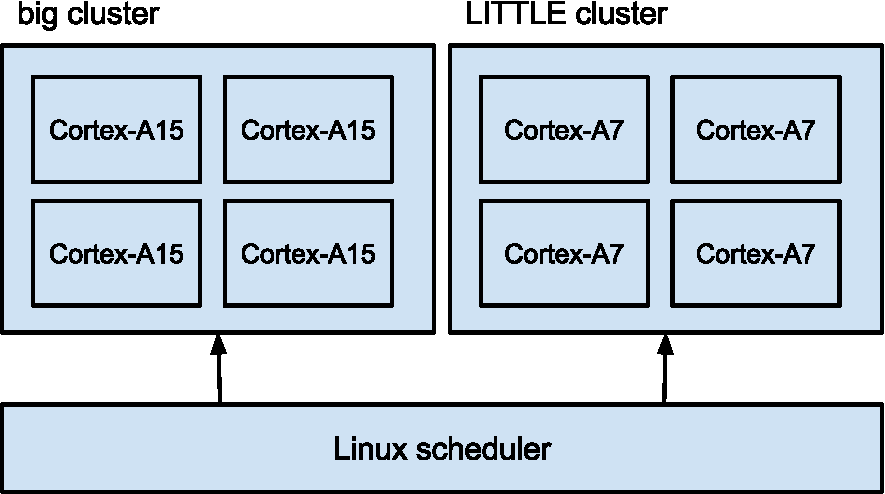
\includegraphics[width=0.6\textwidth]{figs/cluster_switching.pdf}
  \caption{Cluster Switching}\label{cluster_switching}
\end{figure}

\subsection{CPU Migration}

With CPU migration, each big core is paired with a LITTLE core and the OS treats them as a single
core. Like cluster switching, only half the of CPU cores are available at a time but with CPU
migration it can be any combination of big cores and LITTLE cores. The advantage of this approach
over cluster switching is that if the load on the system is only large enough so that a single big
core is needed then power isn't waisted because only a single big core will be switched on. The diagram
in figure \ref{cpu_migration} shows the setup of cpu migration.

\pagebreak

\begin{figure}
  \centering
  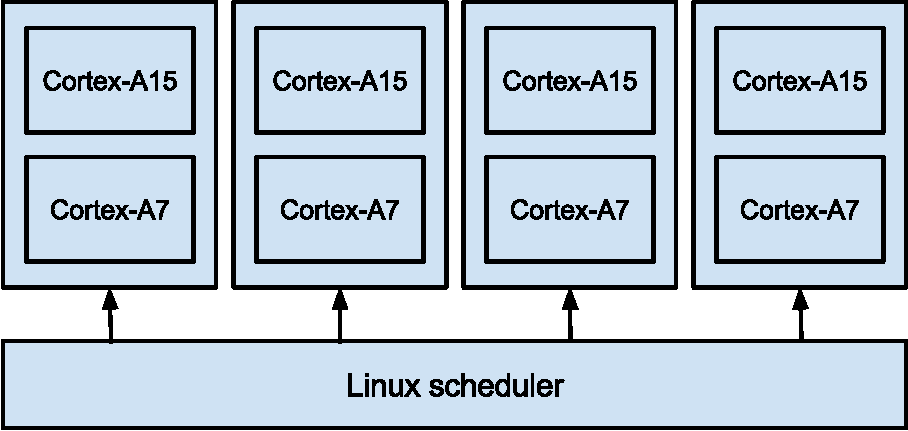
\includegraphics[width=0.6\textwidth]{figs/cpu_migration.pdf}
  \caption{CPU Migration}\label{cpu_migration}
\end{figure}

\subsection{Heterogeneous Multi-Processing (HMP)}

Heterogeneous Multi-Processing or Global Task Scheduling (GTS) allows scheduling to all CPU cores
at the same time. The tasks that have a higher priority or require more processing power will be
scheduled to the big cores whereas the tasks with low priority that don't require much processing
power, such as background tasks can be scheduled to the LITTLE cores. A diagram showing HMP is shown
in figure \ref{global_task_scheduling}.

\begin{figure}
  \centering
  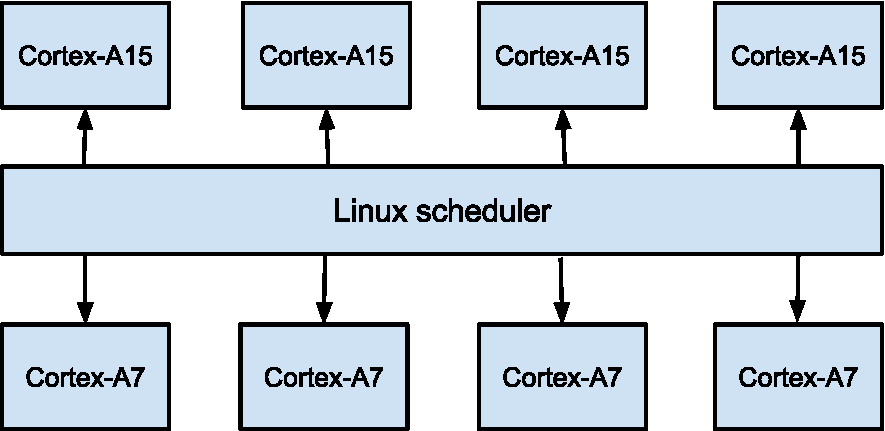
\includegraphics[width=0.6\textwidth]{figs/global_task_scheduling.pdf}
  \caption{Heterogeneous Multi-Processing}\label{global_task_scheduling}
\end{figure}

\section{ODROID XU3}

\begin{figure}
  \centering
  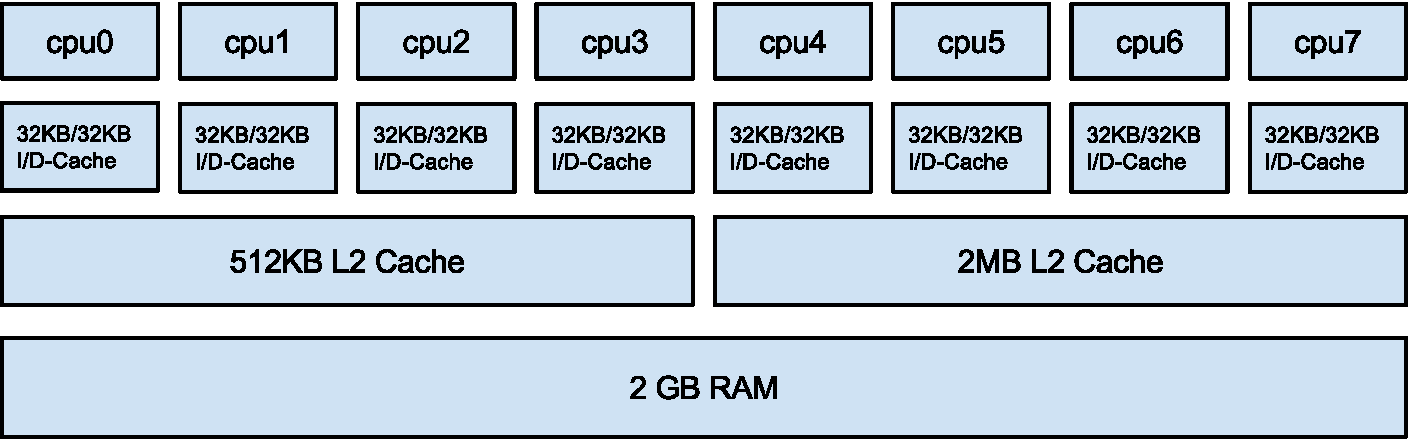
\includegraphics[width=0.6\textwidth]{figs/Odroid-Cache-Hierarchy.pdf}
  \caption{Cache Hierarchy on Exynos 5422 SoC}
\end{figure}

%% ======================================================================================================

\chapter{Related Work}\label{related_work}

This chapter give an overview of some of the most popular Time Warp systems. For each one of the
Time Warp systems a general overview including the main features will first be discussed. Then
the strengths and weaknesses will be detailed as well as the tradeoffs that influenced the design
decisions made while developing the system. Throughout the chapter, the terms message and event
will be used interchangeably.

%% ------------------------------------------------------------------------------------------------------

\section{Georgia Tech Time Warp (GTW)}

Georgia Tech Time Warp is a well-known Time Warp Simulator designed specifically for shared-memory
multiprocessors. Each LP is mapped to a thread which is bound to a single processor in the system.
The mapping of LP's must be set up by the simulation model and remains static throughout the entire
simulation.

Every processor in GTW has it's own pending event set for the LP's that are mapped to it. The pending
event set for each processor consists of three main data structures\cite{das-94}:

\begin{enumerate}

    \item The \emph{Message Queue} is a linked list that contains positive messages that are bound
        for the LP's mapped to the owning processor. Access to the message queue must be synchronized
        because it can be accessed by tasks running on any processor.
    \item The \emph{Cancel Queue} is a linked list that serves exactly the same purpose as the
        message queue except that it containes only negative messages(anti-messages).
        Access to this queue must also be synchronized.
    \item The \emph{Event Queue} is used to hold unprocessed and processed events and is directly
        used to schedule events to be processed. The event queue is actually made up of different
        data structures, one for processed events and one for unprocessed events. The processed
        events are contained within a doubly linked list and the unprocessed events are contained
        within a priority queue which can be configured to be either a calendar queue or a skew
        heap depending on a user configuration.

\end{enumerate}

\noindent
When messages are sent between LP's, they are inserted directly in the message queue or the cancel queue
depending on whether they are positive or negative. Each task that runs on a processor first
moves messages from the message queue to the event queue and processes any rollbacks. Then,
the messages from the cancel queue are removed and cancellations and more rollbacks are processed. The
smallest event from the event queue is then processed. This procedure is repeated over over and over
again by all processors. The main event processing loop in GTW is show in figure \ref{gtw_processing}.

\begin{figure}
\centering
\begin{verbatim}

  while(eventQ is not empty) do
    move messages from MsgQ to EvQ and process any rollbacks
    remove anti-messages from CanQ, process annihilations and rollbacks
    remove smallest timestamped message M from EvQ
    processe message M
  end-while

\end{verbatim}
\caption{GTW Main Event Processing Loop\cite{das-94}\cite{fujimoto-94}\label{gtw_processing}}
\end{figure}

\noindent
To avoid accessing the message queues and cancel queues too often, which will cause contention
problems, GTW also supports batch processing which means that multiple messages will be processed
directly from the event queue without adding any new events or processing rollbacks. After the events
are processed they are added to the processed event list as well as a free-list which will be
described below.

Have to partition the LP's in the simulation model poses some problems. First of all, the behavior
of the simulation must be predicted in order to ensure sure that LP's on different processors will
progress their simulation clocks at similar rates. That is, the smallest simulation clock of all LP's
on any given processor should stay very close. If the LP's on some processors get too far ahead of
those on other processors, then a lot of time will be spent rolling back instead of progressing forward.
Because of this, GTW works well for simulation models with LP's that have are very uniform and every
LP progresses their simulation clock with the same pattern. Furthermore, because the events from
different LP's are merged into the same data structures per processor, it's harder to implement
any kind of LP balancing mechanism. Another problem with the LP partioning in GTW is that the simulation
models must be written with the knowledge of how the underlying simulation mechanism is designed
instead of being transparent to the user. Not only that, but the user must understand the features
of the underlying architecture of the machine such as the number of processors.

The states of the LP's can be save using the traditional copy-state saving or incremental state
saving. The model will choose which state variables need to be automatically saved after every event
that is processed and which state variables need to be incrementally saved. The state variables must
then be registered with the simulation kernel so that they can checkpointed when needed and restored
when a rollback occurs.

Like the pending event set design, the state saving mechanism also forces the user to understand
the underlying simulation mechanism. If a state variable is updated for every event then it is
usually better to always checkpoint to avoid having to keep track of when it gets modified. On the
other if a state variable is not updated frequently, then only saving it incrementally can reduce
the memory footprint of the simulation. The user must understand these tradeoffs and decide which
state saving variables are better for copy-state saving or incremental saving.

GTW does not use conventional fossil collection. Instead, after an event is processed it is added to a
free list of events which is kept by each processor. Events can then be allocated from the free list
as long as the first event in the list has a timestamp less than the GVT. If it is not then the
current event is aborted and fossil collection is initiated. This mechanism is known as "on-the-fly"
fossil collection. One benefit to on-the-fly fossil collection is that it provides a mechanism to
prevent some LP's from processing events too far in the future.

On-the-fly fossil collection was the biggest problem in GTW because it can cause unstable behavior.
As rollbacks occur, the free-list's can become unordered and the first event in the list may not
have a timestamp less than the GVT even if another event in the list does. If a processor tends to
have LP's that rollback more often, then a lot of events can be unnecessarily aborted. Searching
the free-list will not help because it will take more time to search longer lists which will have
the same effect as aborting events. The only way to fix the problem is to allocate much more memory
per processor than is expected to be used.

To calculate GVT, GTW uses an extremely efficient shared-memory algorithm which will be described
in more detail in chapter \ref{gvt_fossilcollection}.

GTW versions only exist for SparcStation and SGI PowerChallenge architectures.

%% ------------------------------------------------------------------------------------------------------

\section{Clustered Time Warp (CTW)}

Clustered Time Warp (CTW) uses a hybrid approach by processing events within a \emph{cluster} of
LP's sequentially and using the Time Warp mechanism between the clusters. This design was chosen
because it works well for digital logic simulation which tend to have localized computation within
a group of LP's. Furthermore, digital logic simulation tends to have low computational granularity
and lot's of LP's which can lead to a lot rollbacks of rollbacks and a large memory footprint in
a traditional Time Warp simulator.

Each cluster has a timezone table, an output queue, and a set of LP's which each have an input queue
and a state queue. The timezones in the timezone table are based on the timestamps of the events
received from LP's on different clusters. Only a single output queue is needed per cluster because
anti-messages can only be sent between clusters and not between LP's on the same cluster. When an
event is received at a cluster a new timezone is created. If the new event is a straggler event then
all LP's that have a larger simulation clock are rolled back. This process of rolling back a group
LP's is known as a \emph{clustered rollback}.

CTW uses a form of infrequent state savings with the timezone table used to determine the frequency.
When an event is about to processed for an LP, the timezone of the last processed event is looked up
and if event that is about to be processed is in a different timezone then the state is saved.
This can significantly reduce the amount of states that needs to be saved if the interactions
between clusters is infrequent.

CTW works well for very specific types of simulations models such as digital logic simulations,
which can be partitioned into seperate functional units. Each of the functional units are very tightly
synchronized and cascading rollbacks can be devastating. This is often not the case with other
simulation models. If the LP's of a simulation model interchange events with only a few other LP's
and stay independent with respect to all others then CTW will not fully exploit the potential
parallelism of the model.

%% ------------------------------------------------------------------------------------------------------

\section{Rensselaer's Optimistic Simulation System (ROSS)}

ROSS is a simulator that is capable of running both conservatively and optimistically synchronized
parallel simulations as well as sequential simulations. It is most often used for optimistically
synchronized simulations which is implemented using the time warp mechanism. ROSS started as a
reimplementation of GTW and is still modeled after it but has some enhancesments. The same basic
event scheduling mechanism is used but ROSS supports different priority queue implementations and
different algorithms are used for fossil collection, state saving, and gvt calculation. In addition,
ROSS uses processes instead of threads and uses MPI to communicate among processes. By using MPI to
communicate among processes, ROSS can be run on a shared-memory multiprocessor, or a cluster, or a
combination of both.

Just as in GTW, ROSS maps every LP to a processor and each processor contains its own pending event
set structures. However, with ROSS each process is assigned to a processor instead of threads and the
processors do no have to be on the same machine. No locks are needed explicity within each process
but rely on the underlying MPI implementation to synchronize access to shared memory. The data structures
are very similar to those used in GTW but have a different naming convention. The main data structures
in ROSS are listed below:

\begin{enumerate}

    \item The \emph{Event Queue} is analogous to the message queue in GTW. It contains the positive
        events for all LP's in the corresponding process. In addition, an event queue is used to
        hold all remote events regardless of whether it is positive or negative. The event queue is
        implemented as a linked list.
    \item The \emph{Cancel Queue} is a linked list which is used to hold negative events for all
        LP's for the corresponding process. The cancel queue is used in the exact same way as GTW
        except that no locks are necessary.
    \item The \emph{Priority Queue} is analogous to the event queue in GTW and contains events in
        timestamp order. ROSS also allows the priority queue to be implemented as a calendar queue,
        heap, splay tree, or avl tree depending on user configuration.

\end{enumerate}

\noindent
The main event processing loop is shown in psuedocode in figure \ref{ross_loop}.

\begin{figure}
\centering
\begin{verbatim}

  while(prQ is not empty) do
    move event from EvQ to PrQ and process any rollbacks
    remove anti-messages from CanQ, process annihilations and rollbacks
    remove smallest timestamped event E from PrQ
    processe event E
  end-while

\end{verbatim}
\caption{ROSS Main Event Processing Loop\label{ross_loop}}
\end{figure}

ROSS does not save any of the LP's state, but instead uses reverse computation to undo erroneous
changes in states. This is 

To calculate GVT, ROSS uses a GVT algorithm called the Seven O'clock algorithm. The Seven O'clock
algorithm makes use of super fined grained cycle counters to synchronize the start of a GVT computation.
Since all distributed processes will have the same cycle counter frequency, the start of the GVT will
be observed by all processes at about the same time. To ensure that messages in transit are counted
and to ensure that clock drift, jitter, and synchronization errors are taken into account, the minimum
value of each process is not computed at the same instant in time that the algorithm is initiated, but
instead each process waits a period of time that is an upper bound on the time it takes to send a
message over the network\cite{bauer-05}.

Because of the limitations of on-the-fly fossil collection, ROSS does not use it and instead uses
conventional fossil collection triggered by a GVT change. To make this more efficient, the processed
events from a group of LP are grouped together in the same data structures. The group of LP's are
known as \emph{Kernel Processes} (KP). In addition to fossil collection, the KP's are also rolled
back as a single unit just as a clustered rollback in Clustered Time Warp.

%% ------------------------------------------------------------------------------------------------------

\section{The ROme OpTimistic Simulator (ROOT-Sim)}

%% ------------------------------------------------------------------------------------------------------

\section{\textsc{warped}}

%% ------------------------------------------------------------------------------------------------------

\section{ROSS-MT}

%% ======================================================================================================

\chapter{The \textsc{warped2} Simulation Kernel}\label{warped2_overview}


%% ------------------------------------------------------------------------------------------------------

\section{The Software Architecture of \textsc{warped2}}

\textsc{warped2} is written in C++ and currently supports sequential simulations and optimistically 
synchronized parallel simulations using the time warp mechanism.

\begin{figure}
  \centering
  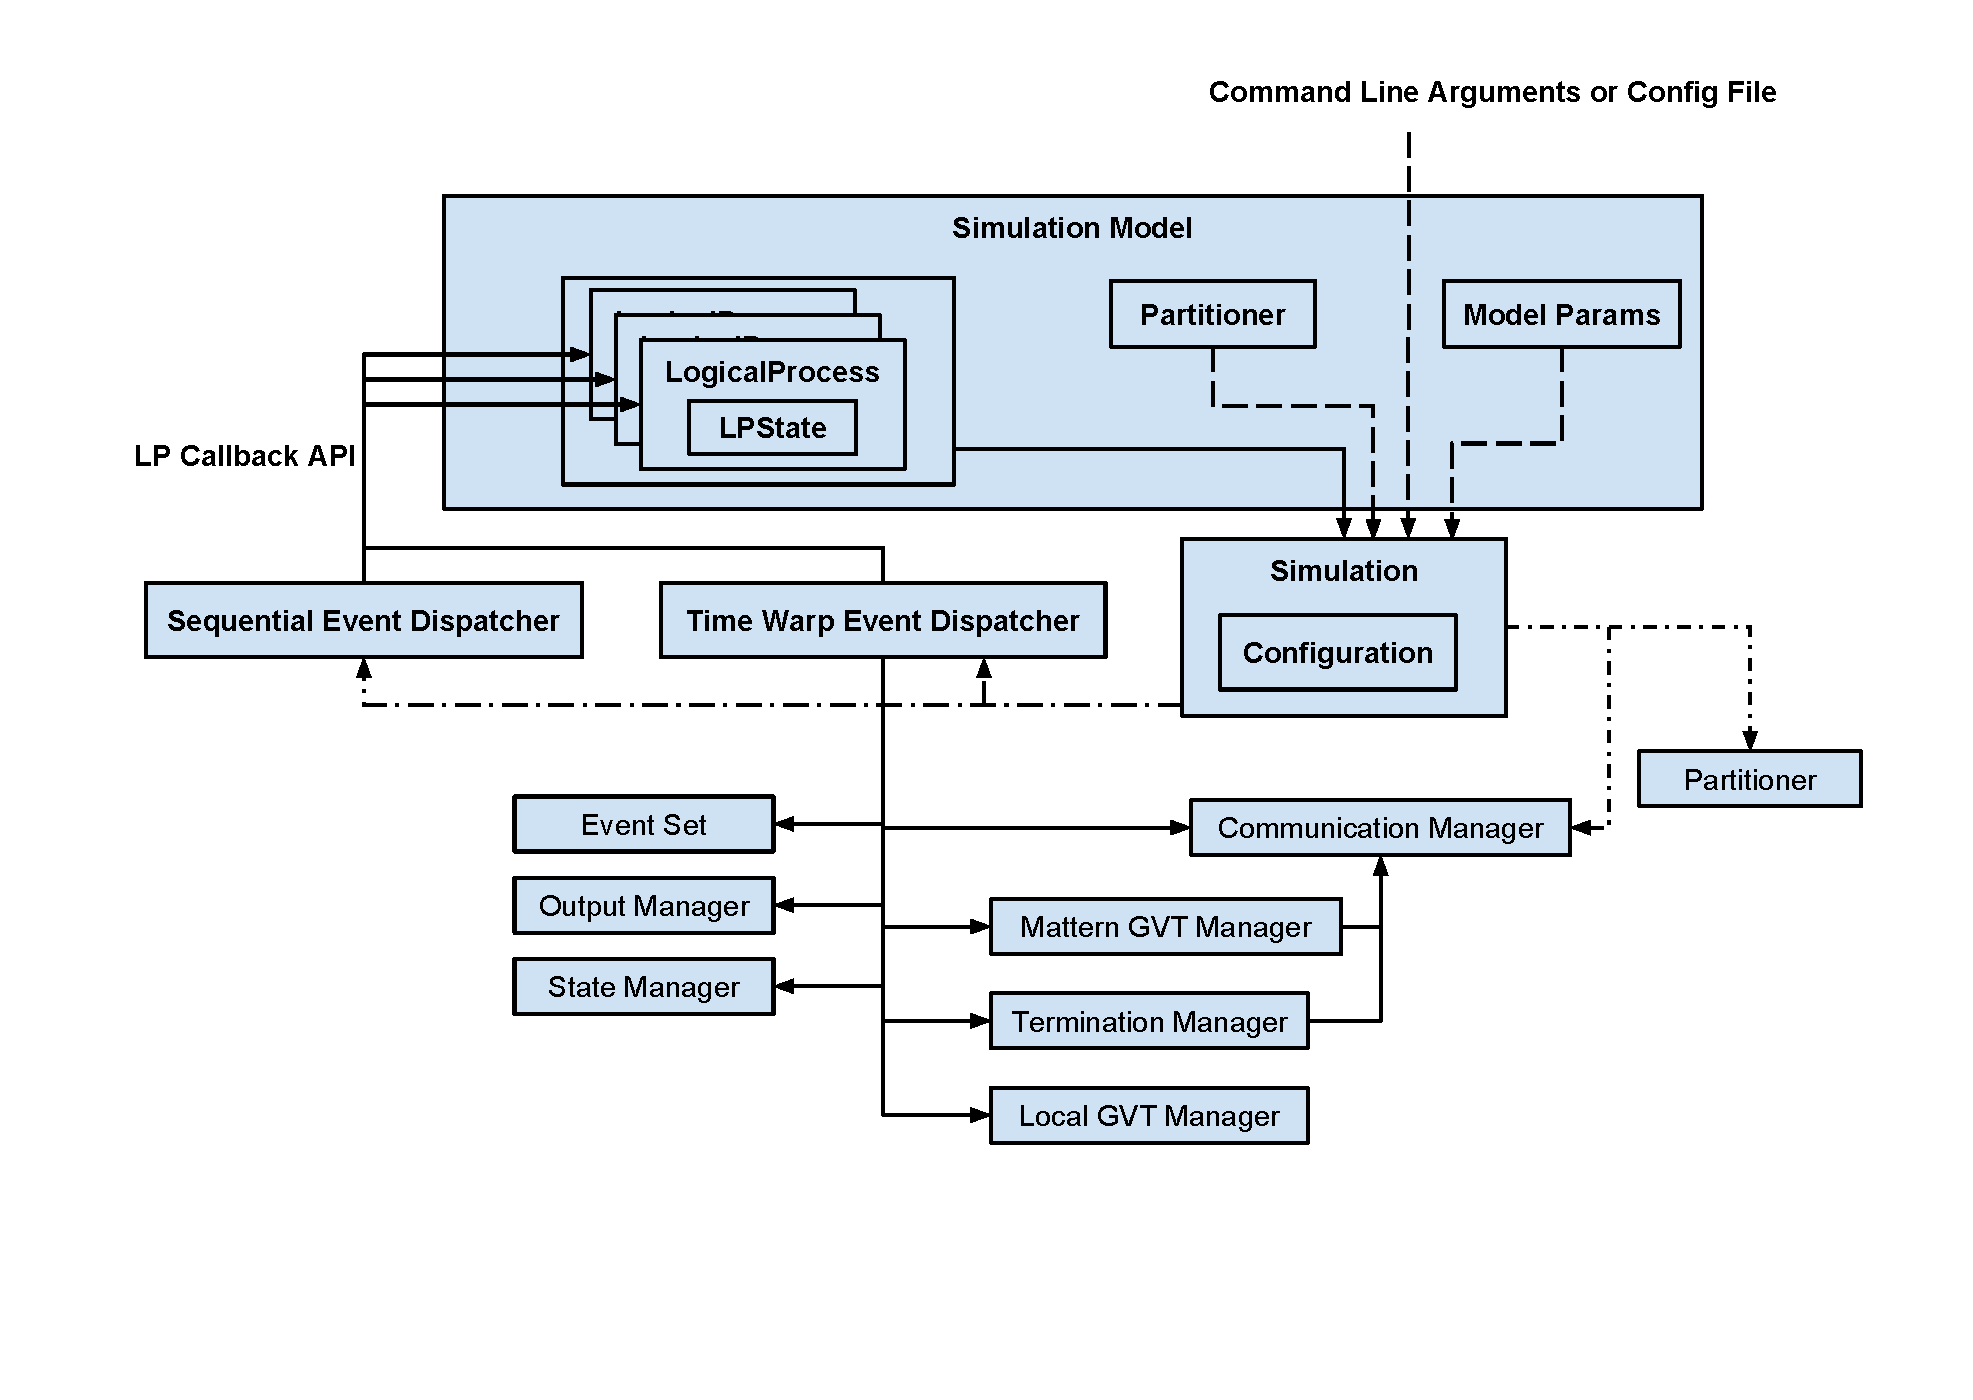
\includegraphics[width=\textwidth]{figs/warped2.pdf}
  \caption{Archicture of \textsc{warped2}}\ref{warped2_architecture}
\end{figure}

The parallel simulations can be configured to run with any number of threads and any number of
processes which can run any number of nodes. Shared memory is used exchange events between LP’s
within the same processes and message passing using is used to exchange event between processes.


\begin{figure}
  \centering
  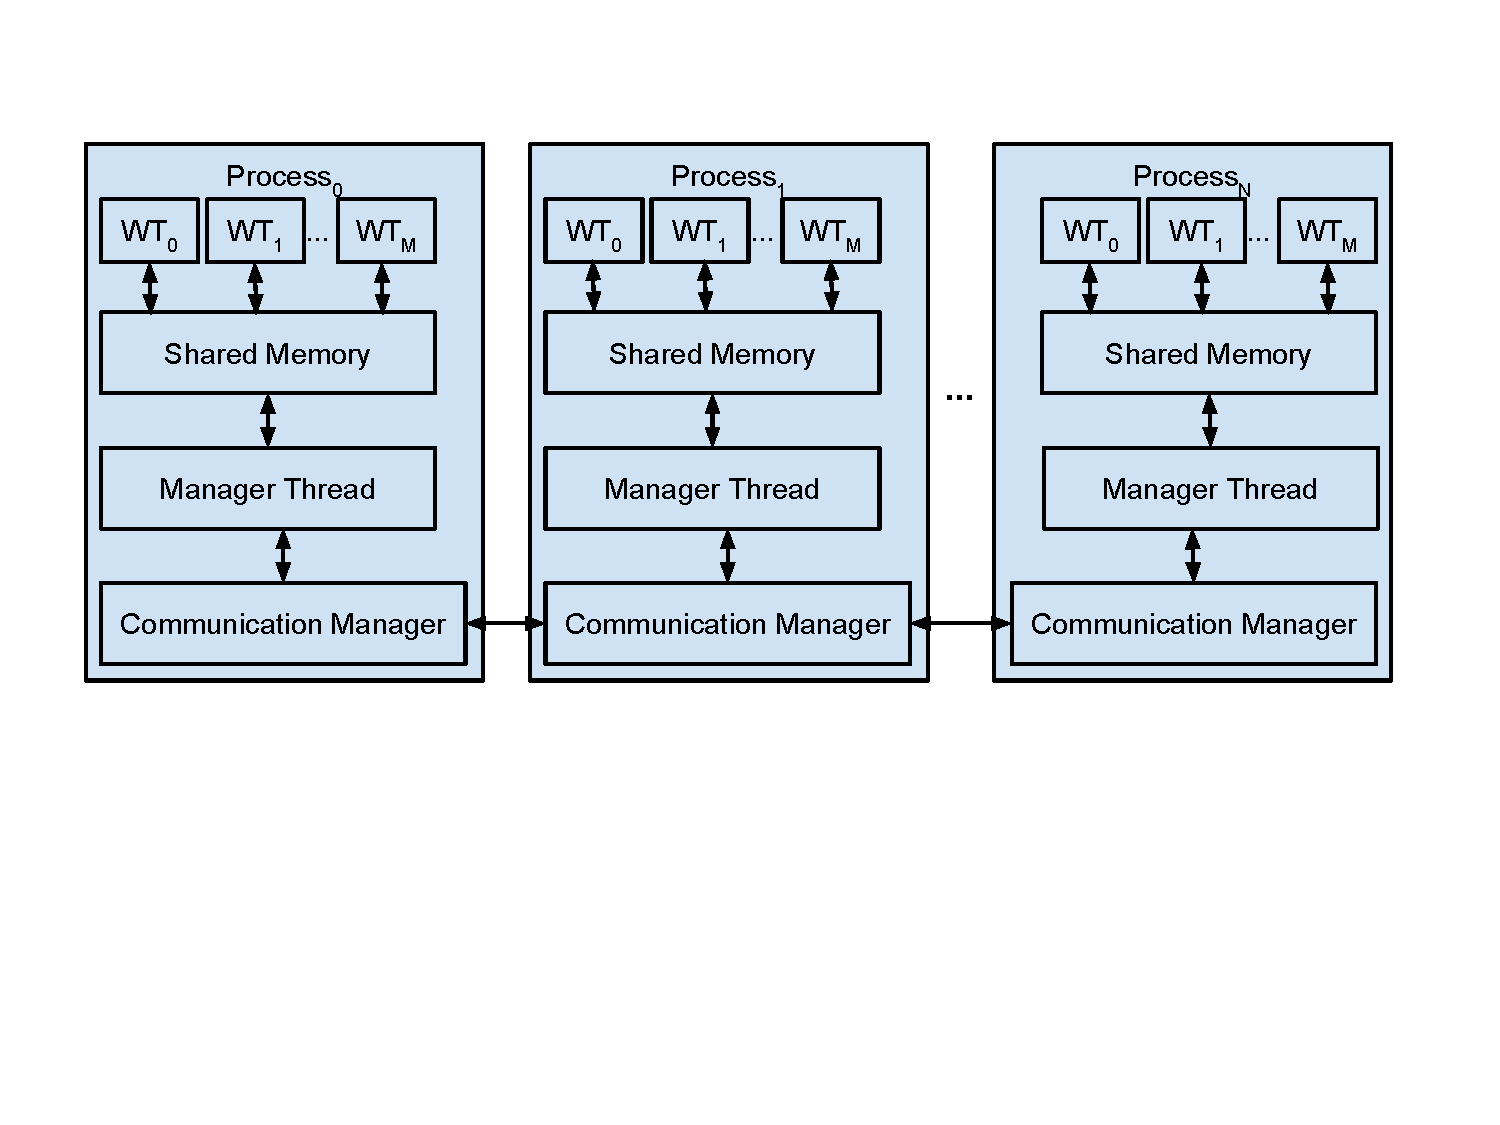
\includegraphics[width=0.6\textwidth]{figs/Warped2-Communication.pdf}
  \caption{Communication Model of \textsc{warped2}}\ref{warped2_communication}
\end{figure}

%% ------------------------------------------------------------------------------------------------------

\section{The Modeling API of \textsc{warped2}}

The modeling interface of warped2 is a set of abstract base classes that contain methods
that must be implemented in a derived class. The base classes may also contain methods and data
members that are available to use by the derived classes. The three main base class types that must
be implemented are LogicalProcess, LPState, and Event. Optionally, the user may create a
custom partitioner from the Partitoner base class. In the remainder of this section, each class
is described in more detail and sample implementations are shown for each.

\subsection{The LPState Structure}

The state of the LPls must be define with the \textsc{warped\_define\_lp\_state\_struct} macro. This
is used to ensure that the warped2 kernel can save a copy of the state and restore the state from
a pointer to the LogicalProcess base class. An intermediate template class is defined which defines
the necessary methods to make a copy of the state and to restore the state so that the user does
need to explicitly define them. However, if the state contains complex data structures
that contains pointers then the default copy constructor and default copy assignment operator will
only perform shallow copies. In this case the user must implement a custom copy constructor
or a custom copy assignment operator or both. The copy constructor will define the behavior for
saving the state whereas the copy assignent operator will define the behavior for restoring the
state. Note that the copy assignment operator will most likely not be needed since a shallow copy
will usually suffice. A simple example of a LP state that contains just message counts is shown
below in listing \ref{sample_state}.

\begin{lstlisting}[caption=Sample \textsc{warped2} State Definition, label=sample_state, float]
WARPED_DEFINE_LP_STATE_STRUCT(SampleState) {
    unsigned int messages_sent_;
    unsigned int messages_received_;
};
\end{lstlisting}

\subsection{The Event Class}

The event base class is used as the basis for creating model specific events. The user must implement
at least two function: \texttt{receiverName()} and \texttt{timestamp()} so that the name of the
receiver and receive time, respectively, can be obtained for each instance of an event. The user
must also register all member variables with the serialization API so that a storage order can be
defined for events that are sent and received over a network. To do this, the
WARPED\_REGISTER\_SERIALIZABLE\_MEMBERS macro is provided. All member variable must be passed to this
macro as well as \texttt{cereal::base\_class<warped::Event>(this)} to ensure that all members that
are inherited are also serialized serialized. The order that the members are listed is completely
arbitrary and does not matter. In addition, the derived event type must be registered using the
WARPED\_REGISTER\_POLYMORPHIC\_SERIALIZABLE\_CLASS macro. A basic sample event implementation is
shown below in listing \ref{event_sample}.

\begin{lstlisting}[caption=Sample \textsc{warped2} Event Definition, label=event_sample, float]
class SampleEvent : public warped::Event {
public:
    SampleEvent() = default;
    SampleEvent(const std::string& receiver_name, const unsigned int timestamp)
                    : receiver_name_(receiver_name), time_stamp_(timestamp) {}

    const std::string& receiverName() const { return receiver_name_; }
    unsigned int timestamp() const { return time_stamp_; }

    std::string receiver_name_;
    unsigned int time_stamp_;

    WARPED_REGISTER_SERIALIZABLE_MEMBERS(cereal::base_class<warped::Event>(this), receiver_name_, time_stamp_)
};
WARPED_REGISTER_POLYMORPHIC_SERIALIZABLE_CLASS(SampleEvent)
\end{lstlisting}

\subsection{The LogicalProcess class}

The most important class definition in the simulation model is the LogicalProcess class. The
implementation of the LogicalProcess class defines the callback functions that the warped2 kernel
calls and thus defines the behavior of the simulation. The user must include a single LPState
implementation as well three method implementations:

\begin{enumerate}

    \item The \texttt{initializeLP} method is called to perform any initializations that must
        be done prior to the start of the simulation and must return a set of initial events.
    \item The \texttt{receiveEvent} method is called to perform some computation based on the event
        that is passed. The implementation of this method interprets the event, updates the state
        of the LP and returns a set of new events with future timestamps.
    \item The \texttt{getState} method provides a way for the warped2 kernel to get the current
        state of the LP.

\end{enumerate}

It is necessary that at least one LP has an initial event that is returned by
initializeLP, otherwise no events can be received and simulation will terminate immediately.
Also note that the it will be called once for \emph{every} LP instance so it is possible that
initial events are returned only in some cases. An example of a LogicalProcess implementation is
shown below in listing \ref{lp_sample}.

\begin{lstlisting}[caption=Sample \textsc{warped2} LogicalProcess Definition, label=lp_sample, float]
class SampleLP : public warped::LogicalProcess {
public:
    SampleLP(const std::string& name, unsigned int initial_events)
        : LogicalProcess(name), initial_events_(initial_events),
          rng_(new std::default_random_engine(rd())) {}

    warped::LPState& getState() { return this->state_; }

    std::vector<std::shared_ptr<warped::Event> > initializeLP() override {

        this->registerRNG(this->rng_);

        std::vector<std::shared_ptr<warped::Event> > events;
        for (unsigned int i = 0; i < this->initial_events_; i++) {
            ++this->state_.messages_sent_;
            events.emplace_back(new SampleEvent { this->get_destination(),
                                            this->get_timestamp_delay() });
        }
        return events;
    }

    std::vector<std::shared_ptr<warped::Event>> receiveEvent(const warped::Event& event) {
        ++this->state_.messages_received_;
        std::vector<std::shared_ptr<warped::Event> > response_events;
        auto received_event = static_cast<const SampleEvent&>(event);
        response_events.emplace_back(new SampleEvent { this->get_destination(),
                                    event.timestamp() + this->get_timestamp_delay() });
        ++this->state_.messages_sent_;
        return response_events;
    }

    SampleState state_;
};
\end{lstlisting}

\subsection{The Partitioner class}

The warped2 kernel already provides a round-robin partitioner and a profile-guided partitioner but
the user can define their own partitioner that is customized for a specific model. The user must
derive from the Partitioner base class and implement just a single method which takes a vector of
all LP'ss and the number of partitions desired and returns a vector of vectors of LP's. In general,
the partitioner should work for any number of partitioners and not impose any constraints because
the partition method is called back from the kernel. A simplified version of the kernel's round-robin
partitioner is shown in listing \ref{partitioner_sample}. Note that a model would never have to
implement such a general partitioner but is showed just as a simple example.

\begin{lstlisting}[caption=Sample \textsc{warped2} Partitioner Definition, label=partitioner_sample, float]
class RoundRobinPartitioner : public Partitioner {
    std::vector<std::vector<LogicalProcess*>>
    partition(const std::vector<LogicalProcess*>& lps, const unsigned int num_partitions) {
        for (unsigned int i = 0, i = 0; i < lps.size(); ++i) {
            partitions[i \% num_partitions].push_back(lps[i]);
        }
    }
};
\end{lstlisting}

\subsection{Random Number Generation}

If the simulation model uses random number generators, they must all be registered with the warped2
kernel. This is necessary so that the state of the random number generator can be saved and restored
in case of rollbacks. The random number generators can be any type as long as they implement the
\texttt{<< operator} and \texttt{>> operator} to allow the kernel to save and restore the internal
state of the random number generator. To register the random number generator, the registerRNG
template function must be used which is a member of the LogicalProcess class. All LP's
must have separate random number generators and must be registered in the initializeLP callback
function as shown in listing \ref{lp_sample}.

\subsection{Command Line Arguments and the Kernel Entry Point}

Once all the necessary structures and classes have been defined, the model's main function must
be implementd which is where all calls into the kernel are made. First, the model specific command
line arguments must be registered with the kernel. This must be done first so that it can be passed
to the constructor of a \texttt{Simulation} instance. Then all of the LP's and optionally a
partitioner must be instantiated and passed to the kernel through the \texttt{simulate}
method of \texttt{Simulation} object. Two versions of the simulate methods are available, one for
a model with a custom partitioner and one without as listed below:

\begin{enumerate}

    \item \begin{verbatim} void simulate(const std::vector<LogicalProcess*>& lps); \end{verbatim}
    \item \begin{verbatim} void simulate(const std::vector<LogicalProcess*>& lps,
                std::unique_ptr<Partitioner> partitioner); \end{verbatim}

\end{enumerate}

\noindent
A sample implementation of a models main function is shown in listing \ref{main_sample}.

\begin{lstlisting}[caption=Sample \textsc{warped2} Main Definition, label=main_sample, float]
int main(int argc, const char **argv) {
    unsigned int num_lps = 10000;

    TCLAP::ValueArg<unsigned int> num_lps_arg("o", "lp-count", "Number of lp's", false, num_lps, "unsigned int");
    std::vector<TCLAP::Arg*> cmd_line_args = {  &num_lps_arg };
    warped::Simulation simulation {"Sample Simulation", argc, argv, cmd_line_args};

    num_lps = num_lps_arg.getValue();
    std::vector<SampleLP> lps;
    for (unsigned int i = 0; i < num_lps; i++) {
        std::string name = std::string("LP_") + std::to_string(i);
        lps.emplace_back(name, 1, i);
    }

    std::vector<warped::LogicalProcess*> lp_pointers;
    for (auto& lp : lps) {
        lp_pointers.push_back(&lp);
    }
    simulation.simulate(lp_pointers);

    return 0;
}
\end{lstlisting}

%% ======================================================================================================

\chapter{Plans of Study}\label{plans_of_study}

%% DOUG: answer the question: ``what are the main points of study''

\section{Implementation components of \textsc{warped2}}

\subsection{Pending Event Set}
%% LTSF queue structures, replication, and LP partitioning

\subsection{State Saving}

\subsection{GVT and Fossil Collection}
%% GVT and fossil collection

%% Mechanisms to Protect Shared Data Structures (spin locks)

%% what else did you/we study

\section{Platforms for Assessment}

\subsection{x86 SMP Nodes and Clusters}

%% ideally you should study a cluster of 16 nodes (8 if 16 not available)

\subsection{ARM big.LITTLE Nodes and Clusters}

\section{Simulation Models used for Assessment}

%% ======================================================================================================

\chapter{Pending Event Data Structures and Their Organization}\label{pending_event_set}

\section{LTSF Replication}

%\showPlots{ltsf_performance.pdf}{ltsf_performance}{Performance of Various Event Set Configurations}

\section{To Thread or Not to Thread}

%% ======================================================================================================

\chapter{State Saving, GVT and Fossil Collection}\label{gvt_fossilcollection}

%% ------------------------------------------------------------------------------------------------------

\section{GVT}

The Global Virtual Time is the minimum timestamp of the unprocessed events in all the pending event
sets and all events that have been sent but not received. The GVT is a global state of the system
which includes the local states of all processes as well as the transient messages. Like all other
global state problems, GVT algorithms are based on basic distributed snapshot algorithms
\cite{chandy-85}\cite{lai-87}\cite{mattern-93} but extended for a particular purpose.

There are two fundamental problems that GVT algorithms must usually solve. The first problem is
known as the \emph{transient message problem}. A transient message is a message that has been sent
but has not yet been received. Careful consideration must be taken to ensure that all transient
messages are taken into account because they can contain timestamped events that are less than all
processes minimum clock. The other problem is called the \emph{simultaneous reporting problem} and
stems from the fact that all processes will not report their minimum clock at the same point in
real time. Because of this, a process can report it's minimum clock value and then receive an event
from a process that has not reported it's minimum clock value, thus missing an event which could have
a lower timestamp.

GVT algorithms can be synchronous which means that all event processing is halted during the GVT 
computation, or asynchronous which does halt event processing. Asynchronous algorithms usually
perform better because the basic computation is not impeded but are much harder to implement due
special cases that must be considered when using message passing concurrently with event processing.

What sets asynchronous GVT algorithms apart is how they handle these two problems. They are a few
main classic asynchronous GVT algorithms that form the basis for other algorithms
Samadi’s\cite{samadi-85} algorithms in the most general form uses acknowledgements for all events
that are received and keeps track of all events sent that have not been acknowledged to solve the
transient message problem. To solve the simultaneous reporting problem, all acknowledgements sent
after the local minimum are marked. The local minimum of each process is then determined by taking
the minimum of the unacknowledged events, the marked acknowledgments sent, and the minimum
simulation clock. Mattern’s algorithm in the most general form uses vector counters to keep track
of the number of events sent and received to and from all processes. A token is passed to all
processes which accumulates all counts and on receipt of the token, the process waits until it’s
message count reaches zero and then passes the token. This ensures that no transient messages are
missed. The minimum of the simulation clocks at each process is also accumulated with each circulation
of the token and is used by the token initiator to determine the GVT approximation. To solve the
simultaneous reporting problem, Mattern’s algorithm uses a coloring scheme to create cuts which
are defined by each circulation of the token. The first circulation of the token is meant to mark
each process so that any events received afterward by an unmarked process is recorded. The second
round is necessary to accumulate the minimum timestamp of unmarked events received at marked
processes and is also used by the token initiator to determine the GVT approximation. A lot of
variations and optimizations exist for these algorithms. For example, cumulative acknowledgements
or scalar message counters can also be used which requires slight changes to the GVT algorithm.
Hybrid approaches of these two algorithms have also been proposed.

The algorithms above are designed for message passing systems which use distributed memory and use
techniques that are not required in a shared memory system. In shared memory systems, there is no
such thing as a transient messages because sending an event can be accomplished by inserting an
event directly into the receiver's input queue. Also, no token is necessary because a shared flag
variable can be used to start the GVT algorithm. Fujimoto developed a very fast asynchronous GVT
algorithm for shared memory multiprocessors which uses

One situation that would be well-suited for a synchronous GVT algorithm would be in large
supercomputers that are designed for efficient collective operations such as the blue gene machine.
ROSS, which is a processed based optimistic simulator implements a synchronous GVT algorithm which
first uses a set MPI\_Allreduce operations to ensure all message counts add up to zero and then
another MPI\_Allreduce on the local minimums of all processes to get the GVT.

%\cite{samadi-85}
%\cite{fujimoto-94}
%\cite{bauer-05}

\begin{algorithm}
\DontPrintSemicolon

\textbf{Process variables}\;
\boldmath$ts_{min}:$ Minimum timestamp of event messages received with final color\;
\boldmath$color:$ Current color of the process\;
\boldmath$color_{initial}:$ Intial color of all processes\;
\boldmath$msgcount_{initial}:$ Messages sent minus messages received with initial color\;
\boldmath$msgcount_{final}:$ Messages sent minus messages received with final color\;
\boldmath$clock_{min}:$ Temporary variable to hold accumulated minimum clock from all processes\;
\boldmath$msgcount:$ Temporary variable to hold accumulated initial color message count from all processes\;\;

\textbf{Event Message}\;
$<sender, receiver, mcolor,...>$\;\;

\textbf{GVT Token Message}\;
$<sender, receiver, mclock, msend, mcount>$\;

\caption{Variables and messages used in GVT algoritm}
\end{algorithm}

\begin{algorithm}
\DontPrintSemicolon
\SetAlgoVlined

  \If{$color_{message} = color_{initial}$} {
    $msgcount_{initial} \gets msgcount_{initial} - 1$\;
  }
  \Else {
    $msgcount_{final} \gets msgcount_{final} - 1$\;
    $ts_{min} \gets \min{(ts_{min}, ts_{event})}$\;
  }

\caption{Message Receive Handler for Event Message}
\end{algorithm}


\begin{algorithm}
\DontPrintSemicolon
\SetAlgoVlined

    $mcolor \gets color$\;
    \If {$color = color_{initial}$} {
      $msgcount_{initial} \gets msgcount_{initial} + 1$\;
    }
    \Else {
      $msgcount_{final} \gets msgcount_{final} + 1$\;
    }

\caption{Event Message Send}
\end{algorithm}

\begin{algorithm}
\DontPrintSemicolon
\SetAlgoVlined
\SetKwFunction{SendToken}{SendToken}

  \If{$color = color_{initial}$} {
    $ts_{min} \gets \infty$\;
    \If{$color = WHITE$}{
      $color \gets RED$\;
    } \Else {
      $color \gets WHITE$\;
    }
  }

  $ts_{min} \gets \min{(ts_{min}, msend)}$\;
  $clock_{min} \gets \min{(clock_{min}, msend)}$
  $msgcount \gets msgcount_{initial} + msgcount$\;
  $msgcount_{initial} \gets 0$\;

  calculate local minimum\;

  \SendToken{$i, (i+1) \bmod N, \min{(lvt_{min}, send_{min})}, ts_{min}, msgcount$}\;

\caption{Message Receive Handler for Mattern Control Token: Non-initiator Node}
\end{algorithm}

\begin{algorithm}
\DontPrintSemicolon
\SetAlgoVlined
\SetKwFunction{SendToken}{SendToken}

  \If {$mcount = 0$} {
    $gvtApprox \gets \min{(mclock, msend)}$\;
    send gvt update token to all nodes\;

    \If{$color_{initial} = WHITE$}{
      $color_{initial} \gets RED$\;
    } \Else {
      $color_{initial} \gets WHITE$\;
    }

    $clock_{min} \gets \infty$\;
  } \Else {
    $ts_{min} \gets \min{(ts_{min}, msend)}$\;
    $msgcount \gets msgcount_{initial} + mcount$\;
    $msgcount_{initial} \gets 0$\;

    calculate local minimum\;

    \SendToken{$i, (i+1) \bmod N, lvt_{min}, ts_{min}, msgcount$}\;
  }

\caption{Message Receive Handler for Mattern Control Token: Initiator Node}
\end{algorithm}

%% ------------------------------------------------------------------------------------------------------

\section{Fossil Collection}

%% ------------------------------------------------------------------------------------------------------

\section{Experimental Assessment}

%% ======================================================================================================

\chapter{Protecting Access to Shared Data}\label{protection}

%% ======================================================================================================

\chapter{Other Studies}\label{other}

%% ======================================================================================================

\chapter{Observations with the ARM big.LITTLE Platform}\label{big_little}

%% ======================================================================================================

\chapter{Summary of Results}\label{results_summary}

%% DOUG: wrap up the results, review the main configurations that make sense to the best
%% general performance that one could expect to use.  depending on your principle results,
%% this may have to be broken down into two main parts, one for x86 and one for ARM.

%% ======================================================================================================

\chapter[Conclusions \& Future Research]{Conclusions and Suggestions for Future Research}\label{conclude}



\section{Summary of Findings}



\section{Detailed Conclusions}



\section{Suggestions for Future Work}



%% ======================================================================================================

%%\Appendix
%%\chapter{Appendix A}\label{appendixA}


\bibliography{refs}
\bibliographystyle{ieeetr} \markright{ }

\end{document}
